\documentclass[aps,prd,twocolumn,showpacs,superscriptaddress,groupedaddress,nofootinbib]{revtex4}  % for review and submission
%\documentclass[aps,preprint,showpacs,superscriptaddress,groupedaddress]{revtex4}  % for double-spaced preprint
\usepackage{graphicx}  % needed for figures
\usepackage[caption = false]{subfig}
\usepackage{lipsum}
\usepackage{dcolumn}   % needed for some tables
\usepackage{bm}        % for math
\usepackage{amsmath,amssymb}   % for math
\usepackage{aas_macros}
\usepackage{multirow}
\usepackage{color}
\usepackage{verbatim}
%\usepackage{times}
\usepackage{url}
\usepackage{hyperref}
%\usepackage{natbib}
%\usepackage{epstopdf}
%\usepackage{subcaption}
% avoids incorrect hyphenation, added Nov/08 by SSR

\newcommand{\bs}{\boldsymbol}
\newcommand{\tcb}{\textcolor{blue}}
\newcommand{\tcr}{\textcolor{red}}
\newcommand{\Largr}{\mathcal{L}}

\hyphenation{ALPGEN}
\hyphenation{EVTGEN}
\hyphenation{PYTHIA}
\textheight=700pt
\begin{document}
% The following information is for internal review, please remove them for submission
\widetext
% the following line is for submission, including submission to the arXiv!!
%\hspace{5.2in} \mbox{Fermilab-Pub-04/xxx-E}
\title{Increasing the Fisher Information Content in the Matter Power Spectrum through Lagrangian Space Reconstruction}
\author{Qiaoyin Pan}
\email{panda@mail.nankai.edu.cn}
\affiliation{School of Physics, Nankai University, 94 Weijin Rd, Nankai, Tianjin, 300071, China}
\author{Ue-Li Pen}
\email{pen@cita.utoronto.ca}
\affiliation{Canadian Institute for Theoretical Astrophysics, University of Toronto, 60 St. George Street, Toronto, Ontario M5S 3H8, Canada}
\affiliation{Dunlap Institute for Astronomy and Astrophysics, University of Toronto, Toronto, ON M5S 3H4, Canada}
\affiliation{Canadian Institute for Advanced Research, Program in Cosmology and Gravitation} 
\affiliation{Perimeter Institute for Theoretical Physics, Waterloo, ON, N2L 2Y5, Canada}
\author{Derek Inman}
\affiliation{Canadian Institute for Theoretical Astrophysics, University of Toronto, 60 St. George Street, Toronto, Ontario M5S 3H8, Canada}
\affiliation{Department of Physics, University of Toronto, 60 St. George, Toronto, ON M5S 1A7, Canada}
\author{Hao-Ran Yu}
\affiliation{Canadian Institute for Theoretical Astrophysics, University of Toronto, 60 St. George Street, Toronto, Ontario M5S 3H8, Canada}
\affiliation{Kavli Institute for Astronomy and Astrophysics, Peking University, Beijing 100871, China}

\date{\today}

\begin{abstract}
  Reconstruction techniques are commonly used in cosmology to reduce
  complicated nonlinear behaviours to a more tractable linearized
  system.  We study a new reconstruction technique that uses the
  Moving-Mesh algorithm to estimate the displacement field
  from nonlinear matter distribution. We show the performance of this
  new technique by quantifying its ability to reconstruct linear
  modes. We study the cumulative Fisher information $I(<k_\mathrm{\tcr{n}})$ about  
  the initial matter power spectrum in the matter power spectra in 130 \tcr{N}-body simulations before 
  and after reconstruction, and find that the nonlinear plateau of
  $I(<k_\mathrm{\tcr{n}})$ is increased by a factor of $\sim 50$ after reconstruction, from
  $I \simeq 2.5 \times 10^{-5} /($Mpc $\tcr{h^{-1}})^3$ to
  $I \simeq 1.3 \times 10^{-3}/($Mpc $\tcr{h^{-1}})^3$ at large $k$.
  This result includes the decorrelation between initial and final fields,
  which has been neglected in some previous studies.
We expect this technique to be
  beneficial to problems such as baryonic acoustic oscillations,
  redshift
space distortions and
  cosmic neutrinos that rely on accurately disentangling nonlinear
  evolution from underlying linear effects.
\end{abstract}


%\pacs{}
\maketitle

\begin{section}{Introduction}\label{sec:introduction}  

  Two-point statistics provide complete descriptions of Gaussian
  density fields and can be computed efficiently even for large data
  sets.  However, nonlinear gravitational evolution leads to highly
  non-Gaussian matter distributions which require higher order
  statistics to fully characterize.  Such statistics are
  computationally expensive and can be challenging to map to
  cosmological parameters.  To mitigate these difficulties, it is
  common to transform the matter field in a way that hopefully reduces
  non-Gaussianity.  For example, Gaussianization transforms have been
  used to make the logarithmic distribution more Gaussian
  \cite{bib:Weinberg1992,bib:Mark2009} and wavelet nonlinear Wiener
  filters have been used to separate Gaussian and non-Gaussian
  components of the density field
  \cite{bib:Zhang2011,bib:Yu2012,bib:HarnoisD2013}.
  {\it Reconstruction} techniques \citep{bib:Daniel2007} provide a more
  effective way by converting matter distributions back to an
  earlier stage \citep{bib:HarnoisD2013}.

  The quality of these techniques can be quantified by computing the Fisher
  information \citep{bib:Rimes2006} present in the power spectrum before and after
  reconstruction/Gaussianization.
  \citet{bib:Rimes2006} were the first to study the Fisher information in the nonlinear
  matter power spectrum calculated from $N$-body simulations.  They
  found that the cumulative information has a plateau on translinear scales
  ($k \simeq 0.2-0.8$ $h$/Mpc) due to strong coupling between Fourier
  modes.  Qualitatively, this means that the power spectra on these
  scales give little additional information.  
  \citet{bib:HarnoisD2013} computed the cumulative Fisher information
  for various Gaussianization methods and their combinations
  and found that while mode coupling is reduced, there is not
  necessarily an improvement in the cross correlation between the
  initial density fields and the final nonlinear ones. 

  In studies of Baryon Acoustic Oscillations (BAO), density fields are
  subjected to reconstruction which partially inverts nonlinear
  evolution by applying the negative Zel'Dovich displacement field \cite{bib:Eisenstein2007}.
  The linear density field is
  typically estimated via Lagrangian perturbation theory (LPT)
  using the linear Zel'Dovich displacement $-\nabla_q\cdot\bs\Psi(\bs q)$
  with respect to initial coordiantes $\bs{q}$ \cite{bib:Zel1970}.
  %\citet{bib:Yu2016} studied the true displacement field in $N$-body simulations by tracking 
  %particles from initial to final conditions. They found this $E$-mode, 
  %component of the exact displacement field provides an excellent reconstruction of 
  %the linear density field. 
  \citet{bib:Yu2016} studied the nonlinear $E$-mode clustering in Lagrangian
  space and find that the linear density field can be well recovered by
  the $E$-mode of the real, nonlinear displacement field.
  This $E$-mode reconstruction therefore provides a theoretical 
  target for other reconstruction techniques to be compared with.
  Recently \citet{bib:Zhu2016} described a new reconstruction 
  technique using the Moving-Mesh
  algorithm (MM), first described in \cite{bib:Pen1995,bib:Pen1998},
  to effectively estimate $\bs{\Psi}(\bs{q})$ from only nonlinear
  density fields.  They further showed that even though shell-crossing
  and vorticity are not recovered, linear density modes are still 
  recovered up to scales relevent to the BAO.

  In this paper, we compute the Fisher information recovered after
  using this new reconstruction scheme on 130 independent $N$-body
  simulations, and compared with other methods and unreconstructed
  fields.  The paper is organized as follows.  In \S
  \ref{sec:reconstruction}, we briefly
  describe the computation of the displacement potential using MM
  algorithm. In \S \ref{sec:simulation}, we describe  
  the simulations, implementation of the reconstruction and compare 
  the power spectra and cross correlations before and after reconstruction.  
  In \S \ref{sec:fisherinfo}, we further compute the correlation matrix 
  and Fisher information before and
  after reconstruction.  Finally, in \S \ref{sec:conclusion}, we summarize 
  our results and 
  discuss the effectiveness of the reconstruction and its potential
  applications.


\end{section}



\begin{section}{Implementation and Power Spectra}
  \label{sec:simulation}
  We use \textsc{CUBEP$^3$M} \cite{bib:Harnois2013} to run
  140 simulations with a box size of 600 Mpc/$h$ and $512^3$ particles.
  For these simulations, we use cosmological
  parameters $\Omega_m=0.321$, $\Omega_{\Lambda}=1-\Omega_m=0.679$,
  $h=0.67$, $\sigma_8=0.83$, and $n_s=0.96$.
  The initial conditions are computed by
  transfer function \cite{bib:Lewis2000}
  at $z=100$.
  Zel'dovich
  approximation is used to calculate the displacement and initial velocities
  of particles.

  \begin{figure*}[t!]
    \centering
    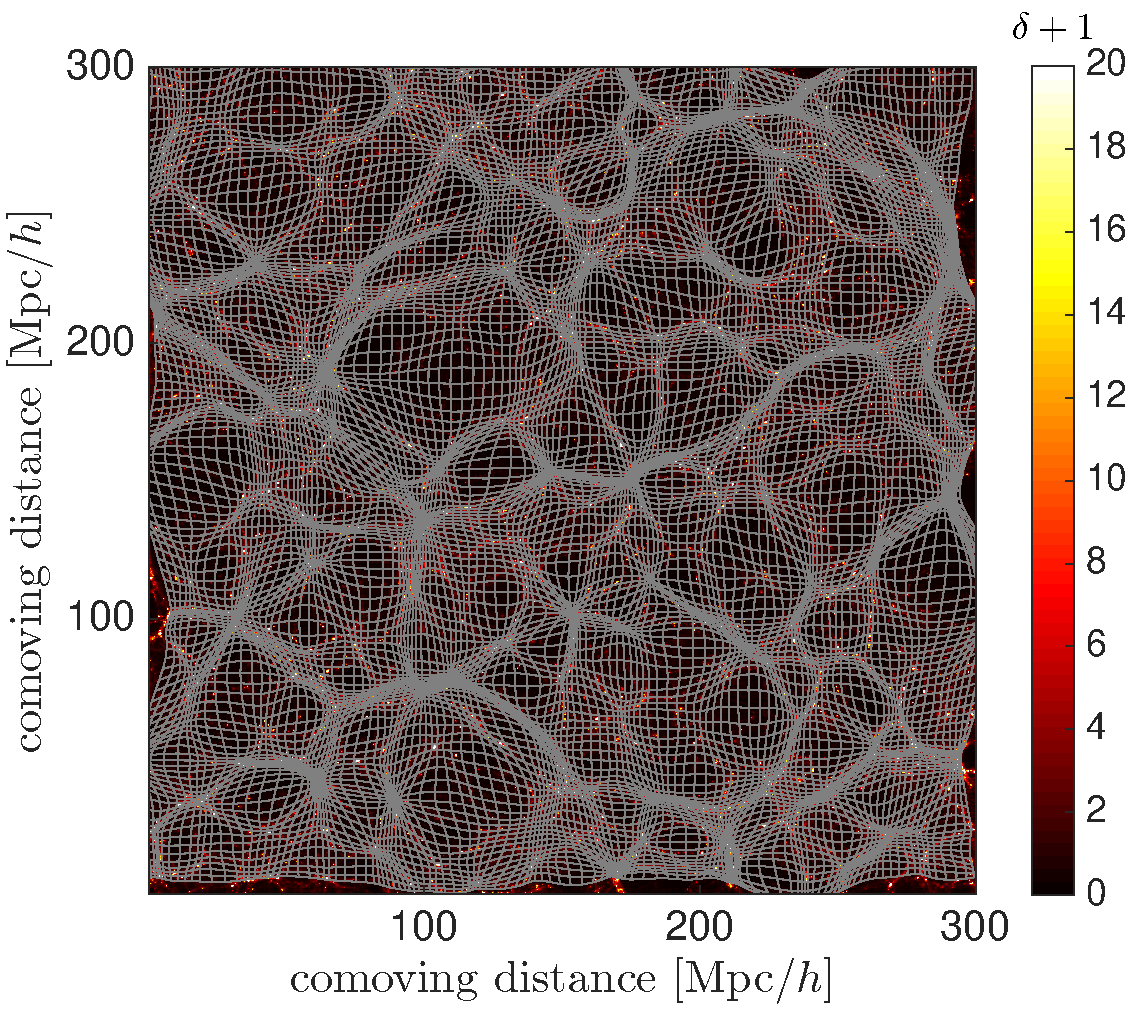
\includegraphics[width=0.9\textwidth]{fig1.pdf}
    \caption{ Illustration of MM reconstruction.
      The 2-D projection of one layer of the deformed mesh of a sample
      $N$-body simulation is shown as curved white lines.  The
      density $\rho/\langle\rho\rangle=1+\delta$ on the mesh is shown
      underneath. For clarity, the scale of the density field is cut to 
      300 Mpc/$h$, and only every other grid line is plotted.}
    \label{fig:simandrec}
 \end{figure*}

 We use the Voronoi tessellation method \cite{bib:Van1994} to estimate the density contrast
 $\delta_N=\rho/\langle\rho\rangle-1$ ($N$ stands for nonlinear) from particle distributions, and apply the
 MM reconstruction to these fields with $512^3$ grids.
 The reconstruction code solves the displacement potentials iteratively
 until the root mean square (rms) of the results drop from $\sim 7.5$
 to 0.20. The compression limiter is set to be 0.1 \cite{bib:Pen1995, bib:Pen1998}. 
 For different simulation samples, a different number of
 iterations are required to get the results of the same rms. A total of
 130 simulations converged to the target rms within 2000 iterations, 
 and we use these results for the calculation in this paper.
 A 2-D projection
 of one layer of the deformed mesh and the original density field on
 the mesh are shown in Fig.~\ref{fig:simandrec}. 
 As expected, the deformed mesh traces the structure very well and
 the deformed grids do not cross each other, even in the 2-D projection.
 
 We study the Fisher information in the matter power
 spectra. More generally,
 the cross power spectrum $P_{\alpha\beta}(k)$ for species $\alpha$ and $\beta$
 ($\alpha=\beta$ for auto power spectrum) is defined as
 \begin{align}
   \langle \delta_\alpha^\dagger(\bm{k})\delta_\beta(\bm{k}') \rangle =
   (2\pi)^3 P_{\alpha\beta}(k) \delta_{\rm {3D}}(\bm{k}-\bm{k}'),
 \end{align}
 where $\delta_{\alpha}$ and $\delta_{\beta}$ are any two fields and
 $\delta_{\rm{3D}}$ is the three-dimensional Dirac delta function. We typically consider instead
 the dimensionless power spectrum, $\Delta_{\alpha\beta}^2(k)$, defined as
 \begin{align}
   \Delta_{\alpha\beta}^2(k) \equiv \frac{k^3 P_{\alpha\beta}(k)}{2\pi ^2}.
 \end{align}
 In the left panel of Fig.~\ref{fig:cp}, we show the matter auto power
 spectrum of linear theory density fields $\delta_L$, nonlinear density
 fields ($\delta_N$) from simulations and reconstructed density fields
 (from Eq. \ref{eq:delta}).  For the simulation
 results, we use the average value of all 130 simulations and show
 $1\sigma$ standard deviations as error bars.  

 To quantify the cross-correlation
 between fields, we compute the cross correlation coefficient
 $r_{\alpha\beta}(k)\equiv P_{\alpha\beta}/\sqrt{P_{\alpha\alpha}P_{\beta\beta}}$.  In the right panel of
 Fig.~\ref{fig:cp}, we show $r_{NL}$ and $r_{RL}$.  We see that, compared with $\delta_N$,
 $\delta_R$ correlates with $\delta_L$ on much wider range of scales.
 We compare our reconstruction correlation coefficient to that of the $E$-mode 
 reconstruction, $r_{EL}$, 
 %,($\delta_E(\bs{q})= - \nabla_q \cdot \bs{\Psi}(\bs{q})$) 
 computed in \citet{bib:Yu2016}.
 Even though $r_{RL}$ decreases from $r_{EL}$ in the nonlinear regime due to the fact that the MM reconstruction 
 cannot recover the shell-crossing present on these scales, we find that linear
 modes are recovered successfully on scales $k\simeq 0.05 - 0.3$ $h$/Mpc.
 Specifically, the scale where $r(k)=1/2$ increases from $k\simeq 0.2$ $h$/Mpc to
 $0.8$ $h$/Mpc after reconstruction.  In comparison with the results of \citet{bib:ZhuH2016},
 which showed $r(k\simeq0.9 h/\rm{Mpc})=1/2$, we find the correlation coefficient falls off at slightly lower
 wave numbers, which we attribute to using fewer particles per simulation.

  \begin{figure*}
    \centering
    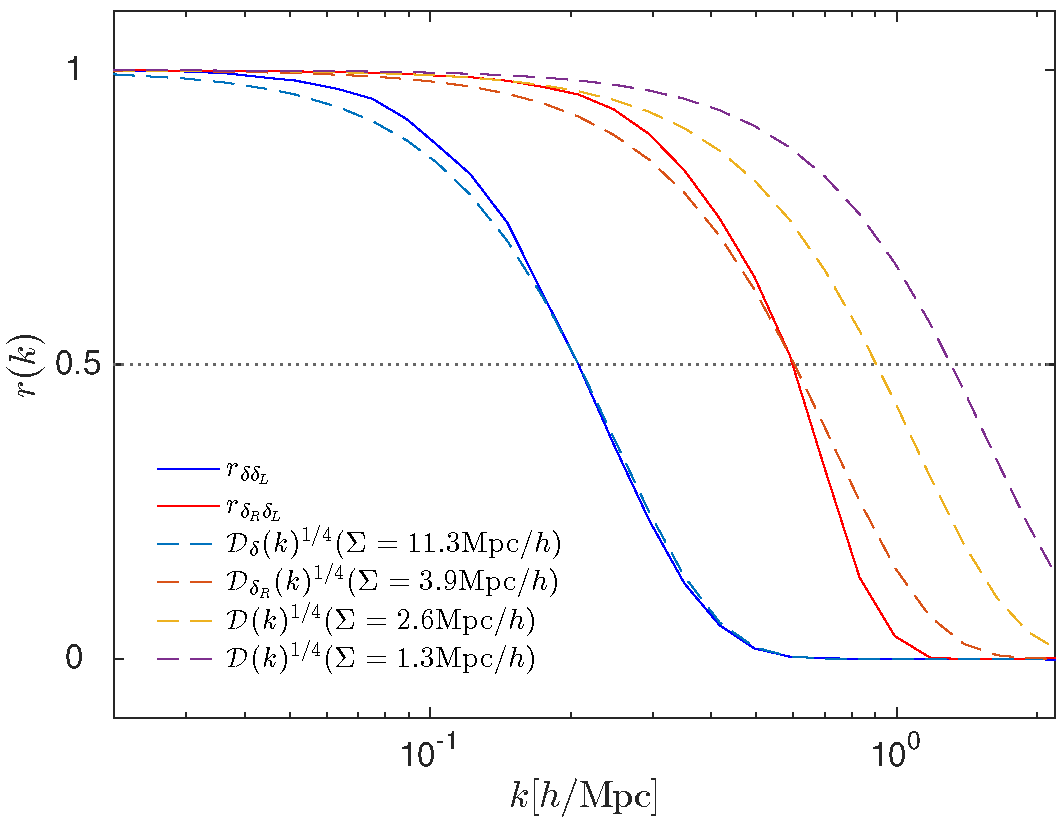
\includegraphics[width=0.5\textwidth]{fig2a.pdf}
    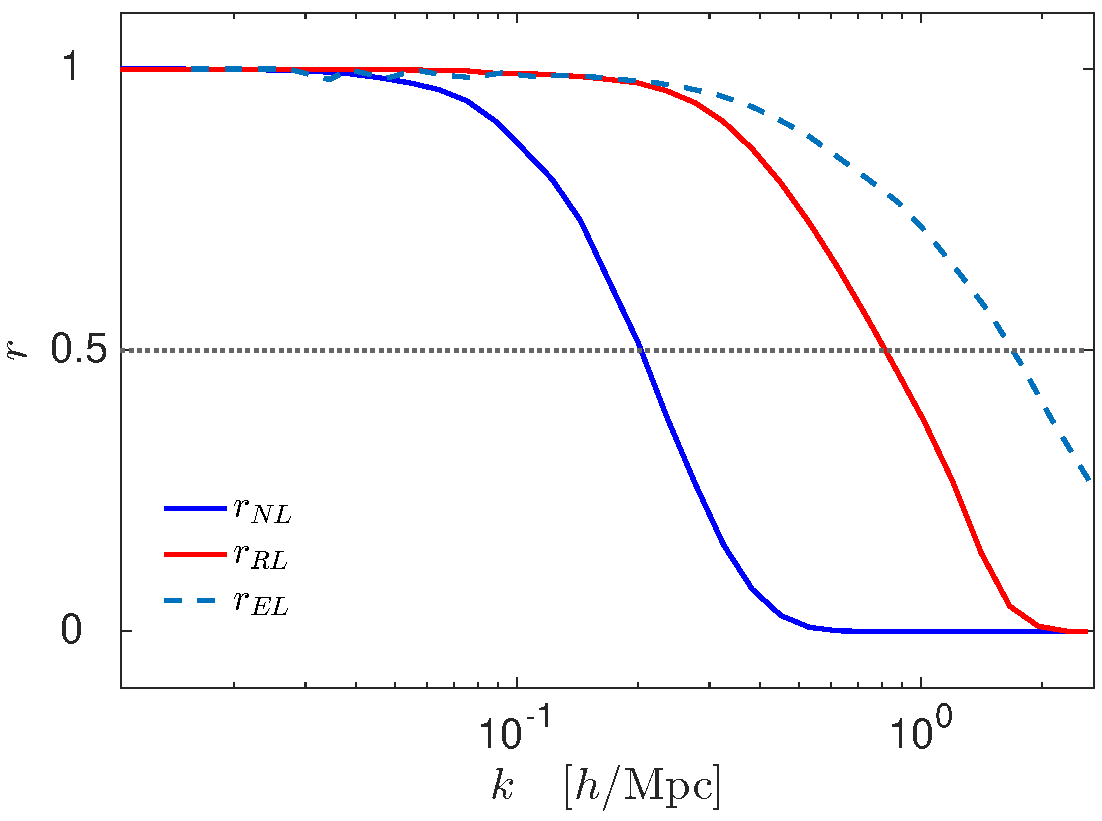
\includegraphics[width=0.485\textwidth]{fig2b.pdf}
    \caption{{\it Left.} The dimensionless power spectrum computed via
      linear theory (black), the mean value of 130 $N$-body
      simulations with $1\sigma$ error bars (blue), and reconstruction
      of the simulations (red).  {\it Right.} The cross correlation
      coefficient between simulation and linear densities $r_{NL}$ (blue),
      MM reconstructed and linear densities $r_{RL}$ (red), and E-mode reconstruction $r_{EL}$ (dashed
      blue) from \citet{bib:Yu2016}.}
    \label{fig:cp}
  \end{figure*}


\end{section}



\begin{section}{Reconstruction Algorithm}
  \label{sec:reconstruction}
   The basic idea of the MM algorithm is to build a PM scheme on a curvilinear coordinate system, 
in which the number of particles per grid cell is set approximately constant. 
    Consider a numerical grid of curvilinear coordinates 
$\bm{\xi}=\left(\xi_1,\xi_2,\xi_3\right)$. In order to determine the physical position 
of each grid point, one needs to specify the Euclidean coordinate $\bm{x}(\bm{\xi},t)$ 
as a function of grid position. In the Euclidean coordinate, the flat metric is the Kronecker 
delta function $\delta_{ij}$, while the curvilinear metric is given by
\begin{align}
    g_{\mu\nu}=\frac{\partial x^i}{\partial \xi ^\mu} \frac{\partial x^j}{\partial \xi ^\nu}\delta_{ij}.
\end{align}
    We use the convention that Latin indices denote Cartesian coordinate, 
while Greek indices denote the curvilinear grid coordinate.
    In principle, there are many different methods to connect the Cartesian 
coordinate and curvilinear coordinate of each grid cell. In the APM method, the 
connection is described by an irrotational deformation,
\begin{align}
    x^i=\xi ^\mu \delta ^i _\mu + \Delta x^i,
\end{align}
where
\begin{align}
 \label{eq:disp}
    \Delta x^i=\frac{\partial \phi}{\partial \xi ^ \nu}\delta ^i _\nu .
\end{align}
    This choice of the deformation can minimize mesh distortion and twisting. $\phi$ is called 
the deformation potential, and $\Delta x^i$ the lattice displacement. The deformation potential 
can be given in terms of the continuity equation in curvilinear coordinates,
\begin{align}
 \label{eq:continue_eq}
    \frac{\partial (\sqrt{g} \rho) }{\partial t}+\partial_\mu \left[\rho \sqrt{g} e^\mu _i \left(v^i - \Delta \dot{x}^i \right) \right] =0
\end{align}
where $\sqrt{g} \equiv \mathrm{det}\left| e^i_\mu\right|$ is the volume element 
and thus $\sqrt{g} \rho$ represents the particle mass in the volume element under the curvilinear 
coordinate system. The triad is given by $e^i_\mu = \partial x^i / \partial \xi ^ \alpha$. 
$\Delta \dot{x}^i=\delta ^{i\nu}\partial _\nu \dot{\phi}$ is chosen such that the first 
term in Eq.\ref{eq:continue_eq} is zero, resulting in a constant mass per volume 
element. The velocity field divergence is replaced by the deviation density field 
$\Delta \rho = \bar{\rho}-\rho \sqrt{g}$, which ideally should be zero. Then the 
deformation potential is described via the elliptic equation,
\begin{align}
 \label{eq:li_elip}
    \partial _\mu (\rho \sqrt{g} e^\mu _i \delta^{i\nu}\partial_\nu \Delta \phi)=\Delta \rho
\end{align}
The Eq.\ref{eq:li_elip} can be solved using multigrid algorithm described in Ref. 
\cite{bib:Pen1995,bib:Pen1998}. The displacement is then given by the gradiant of the deformation 
potential as in Eq.\ref{eq:disp}. We run the MM reconstruction code on 136 non-linear density field from simulation 
in a resolution of ng$=128$ per dimension. The multigrid algorithm is iterated for 1000 times and it rms 
decreases from roughly 4.5 to roughly 0.2. 
A 2-D projection of one layer of the deformed grids and the 
original density field is given in Fig.\ref{fig:simandrec}. 
As expected, there is no grid crossing after reconstruction.
%
\end{section}



\begin{section}{Power Spectra and Information Content}
  \label{sec:fisherinfo}
    The power spectrum is the Fourier transform of the correlation function and measures
 the amount of clustering in the matter distribution as a function of wavenumber $k$,
\begin{align}
    \langle \delta \left( \bm{k} \right) \delta \left( \bm{k'}\right) \rangle =
\left( 2\pi \right) ^3 P \left( \bm{k} \right) \hat{\delta} \left( \bm{k}-\bm{k'} \right),
\end{align}
where $\delta \left( \bm{k} \right)$ is the density fluctuation in wave space, while 
$\hat{\delta}$ is the delta funciton. Of equal interest is $\Delta ^2_k$, the power 
spectrum in its dimensionless form, defined as
\begin{align}
    \Delta ^2(k) \equiv \frac{k^3 P \left( k \right)}{2\pi ^2}
\end{align}
    The power spectra of the mass distributions are calculated using the \enquote{Nearest Grid Point} 
(NGP) mass assignment scheme. In Fig. \ref{fig:cross-correlation-power}(a) we plot the mean cross correlation 
function, $r=P_{\delta \delta_L}/\sqrt{P_\delta P_{\delta_L}}$ of the non-linear and the 
linear power spectrum, and the reconstructed and 
linear power spectrum respectively. The wave number where the cross correlation drops to a half increases 
from $k\simeq$ 0.2 $h/\mathrm{Mpc}$ to $k \simeq$ 0.6 $h/\mathrm{Mpc}$. 
To qualify the improvement of cross correlation in the 
power spectrum, we compute the damping factors $\mathcal{D}(k)=r^4$ fitting the Gaussian BAO damping models 
$\mathcal{D}(k)=\mathrm{exp}(-k^2 \Sigma^2/2)$. In Fig. \ref{fig:cross-correlation-power}(a) 
we plot $\mathcal{D}_\delta^{1/4}$ ($\Sigma =$ 11.3 $\mathrm{Mpc}/h$) and $\mathcal{D}_{\delta_R}^{1/4}$ 
($\Sigma = $ 3.9 $\mathrm{Mpc}/h$) over $r_{\delta\delta_L}$ and $r_{\delta_R\delta_L}$. 
We also plot the $r_{\delta\delta_L}$ and $r_{\delta_R\delta_L}$. We also plot $\mathcal{D}(k)^{1/4}$ 
that match cross correlation function after $E$-mode displacement 
reconstruction ($\mathrm{ng}=512$, box size=400 $\mathrm{Mpc}/h$, $\Sigma =$ 1.3 $\mathrm{Mpc}/h$), 
which is the result in \cite{bib:Yu2016} and 
MM reconstruction in a higer resolution ($\mathrm{ng}=512$, box size=600 $\mathrm{Mpc}/h$, $\Sigma =$ 2.6 $\mathrm{Mpc}/h$), 
which is the result in \cite{bib:ZhuH2016}. We find that with higher resolution, which is more precise, 
the reconstruction gives a cross correlation damping at smaller scale. 
And it's expected that the $E$-mode displacement reconstruction gives a reconstructed power spectrum more correlated 
with the initial one, since it decomposes completely the irrotational and curl components of the real displacement 
field in N-body simulation, while the difference between the reconstructed displacement through MM reconstruction 
and the real displacement still has an irrotational component.
 In Fig. \ref{fig:cross-correlation-power}(b) we plot the linear power spectrum which is the transfer function, and mean 
power spectrum (with error bars) of 136 non-linear density fields and reconstruced density fields simply 
given by $\delta_R=\bm{k}\cdot\bm{k}\xi$. The reconstructed power spectrum drops at non-linear scale ($k \gtrsim$ 0.3 $h/\mathrm{Mpc}$) 
since the reconstructed density fields are totally irrotational. The result is similar to that of 
E-mode displacement reconstruction described in \cite{bib:Yu2016}, in which the reconstructed power spectrum 
drops, but in a different scale and at a different speed.
\begin{figure*}
%\begin{subfigure}[b]{0.48\textwidth}
\centering
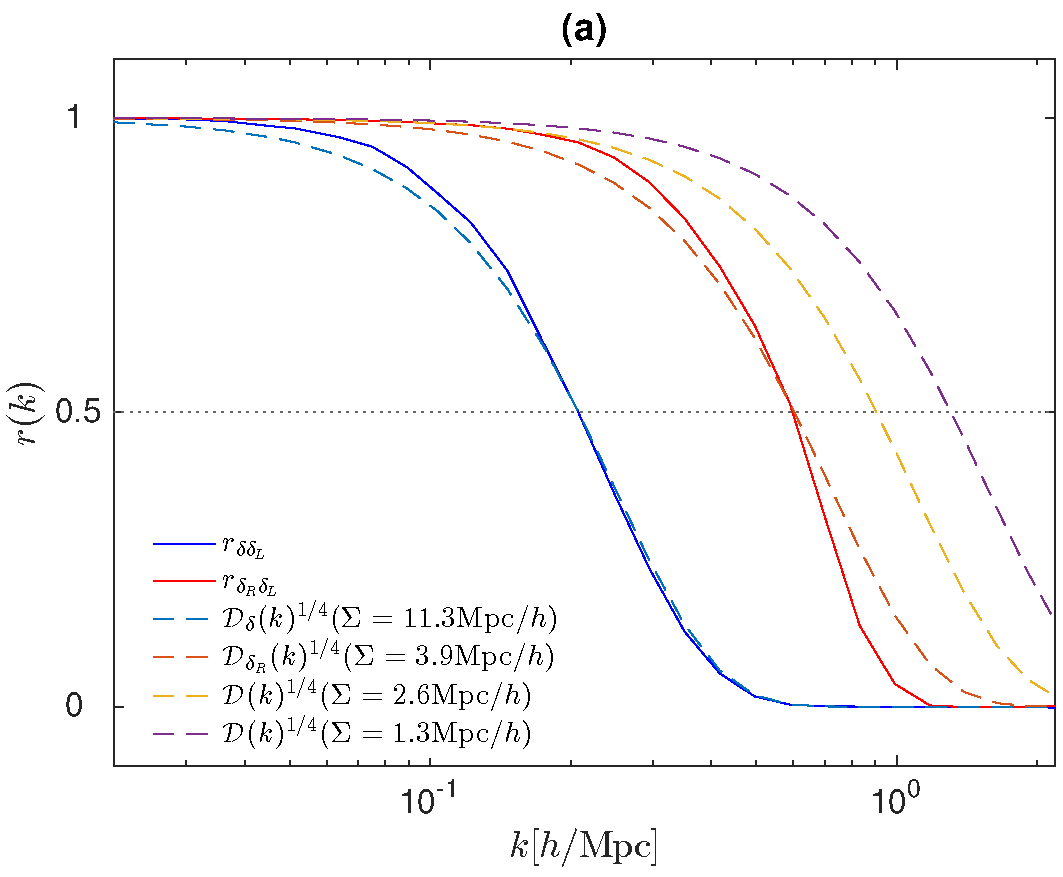
\includegraphics[width=0.455\textwidth]{cross_correlation_best_analysis-crop.pdf} 
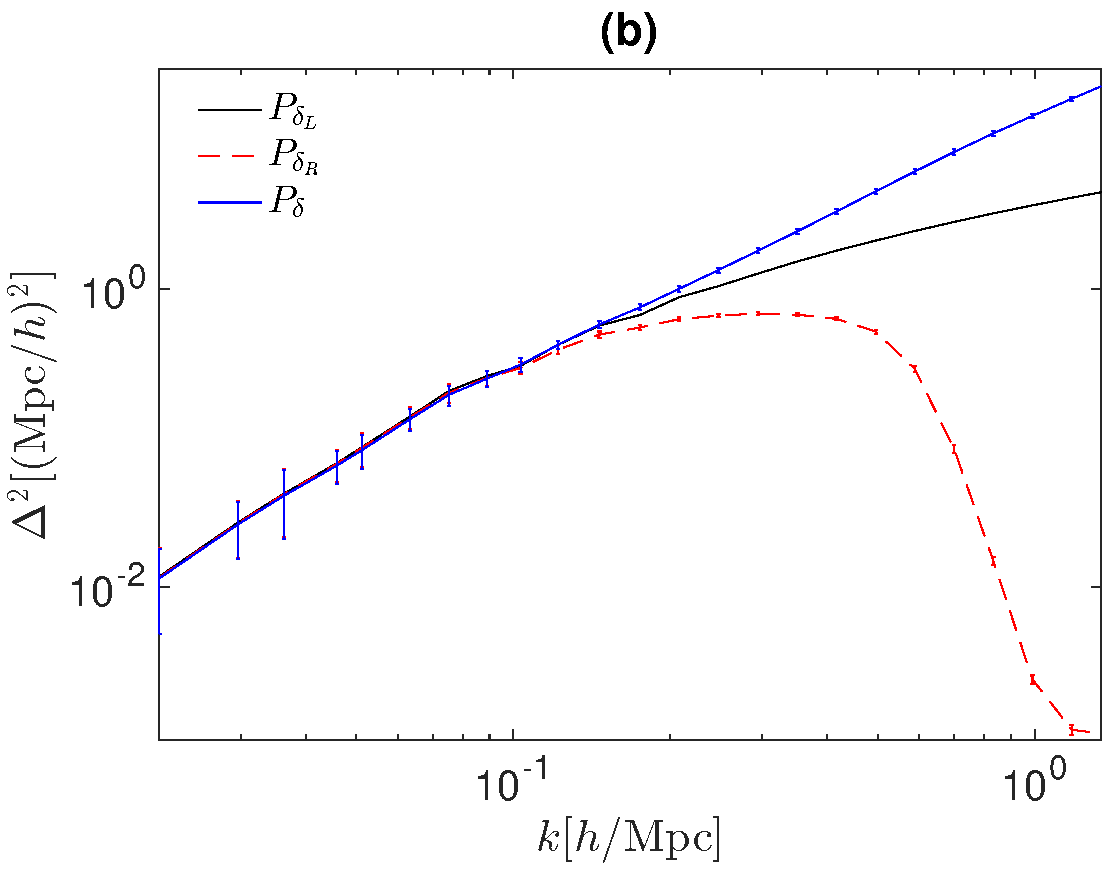
\includegraphics[width=0.48\textwidth]{power_best_analysis-crop.pdf}
%\includegraphics[width=0.5\textwidth]{power_nberror-crop.pdf}
\caption{(a) The cross correlation function (solid lines) $r(\delta,\delta_L)$ (blue) and $r(\delta_R,\delta_L)$ (red), 
and BAO damping models (dash lines). 
(b) The dimensionless power spectrum computed via linear theory (black), the mean value of 136 $N$-body simulations
with $1\sigma$ error bars (blue), and reconstruction of the simulations (red).}
\label{fig:cross-correlation-power}
\end{figure*}

   Mathamatically, the Fisher information \cite{bib:Tegmark1997} $I$ in the log of amplitude $A$ of the initial 
matter power spectrum is defined as 
\begin{align}
   I_A \equiv -\left\langle \frac{\partial ^2 \mathrm{ln \Largr}}{\partial A ^2}\right\rangle,
\label{eq:fisherdefine}
\end{align}
   in which $\Largr$ denotes the likelihood. For Gaussian fluctuations, the likelihood depends on
parameters only through the power spectrum $P(k)$, and the information $I$ in A defined by Eq. \ref{eq:fisherdefine}
can be written as \cite{bib:Rimes2006}
\begin{align}
    I_A = - \left\langle \sum_{k,k'} \frac{\partial \mathrm{ln} P(k)}{\partial \mathrm{ln} A} 
\frac{\partial ^2 \mathrm{ln \Largr}}{\partial \mathrm{ln} P(k) \partial \mathrm{ln} P(k')}
\frac{\partial \mathrm{ln} P(k')}{\partial \mathrm{ln} A}\right\rangle,
\label{eq:fisherdefineforgaussian}
\end{align}
in which the angle bracket denotes the average over all the power spectra.

  The definition Eq. \ref{eq:fisherdefineforgaussian} can be written in a simpler form in two aspects, one 
of which is the first and the third partial dericative terms. 
For any density field $\delta$, we can conveniently decompose it into linear and non-linear components
\begin{align}
    \delta (k) = b (k) \delta _L (k) + n (k),
\label{eq:decompose}
\end{align}
in which $\delta_L$ denotes the linear density field. $b (k)$ is the bias and $n (k)$ is defined  
such that the correlation $\langle \delta_l (k) n (k) \rangle$ is zero. If we correlate  
$\delta$ and $\delta_L$,
\begin{align}
   \langle \delta (k) \delta_L (k) \rangle = b (k) \langle \delta_L (k) \delta_L (k) \rangle,
\label{eq:correlating}
\end{align} 
    we can solve for $b$ as 
\begin{align}
    b (k) = \frac{P _{\delta \delta_L}(k)}{P_{\delta_L}(k)}.
\label{eq:bofk}
\end{align}
Non-linear evolution drives $b (k)$ to drop from unity, and generates the non-linear term $n (k)$. 
Correlating $\delta$ and itself, 
\begin{align}
  \langle \delta (k) \delta (k) \rangle = b^2 (k) \langle \delta_L (k) \delta_L (k) \rangle + \langle n(k)n(k) \rangle,
\end{align}
we find 
\begin{align}
   P_\delta (k) = \mathcal{D} (k) P_{\delta_L} (k) + P_n (k),
\label{eq:powerdecompose}
\end{align}
where $\mathcal{D}(k) \equiv b^2 (k)$ is the non-linear damping factor, and $P_n$ is the mode-coupling term.

   With the help of Eq. \ref{eq:bofk} and Eq. \ref{eq:powerdecompose}, we can replace the partial derivatives 
$\partial \mathrm{ln} p(k) / \partial \mathrm{ln} A$ in Eq. \ref{eq:fisherdefineforgaussian} with 
\begin{align}
   \frac{A}{P(k)}\frac{\partial P(k)}{\partial A}=frac{P_{\delta \delta_L}^2(k)}{P_\delta P_{\delta_L}}
\end{align}
which is just the square of the 
cross correlation function $r ^2 (k)$, of $\delta$ and $\delta_L$. 

The second partial derivative terms in 
Eq. \ref{eq:fisherdefineforgaussian}, the Hessian of the vector $\mathrm{ln} P(k)$, has the expectation 
value of the Fisher matrix with respect to the log powers. For linear density fields, the Fisher matrix is 
approximately equal to the inverse of the covariance matrix of power spectrum estimates, which should be diagonal, 
with diagonal elements equal to the number of modes in each wavenumber bin (when considering $\bm{k}$ and $-\bm{k}$ 
as the same mode). Thus we can write down a simpler matrix product form of cumulative Fisher information, 
\begin{align}
    I_A \left( < k_n\right) = r^2(k)^{\mathrm{T}} \left[ \mathrm{C^{-1}_{norm}} ( k,k' )\right] r^2(k') ,
\label{eq:fisherformulaused}
\end{align}
where $\mathrm{C_{norm}}$ is the normalized covariance matrix with size per dimension up to $k_n$, defined as
\begin{align}
    \mathrm{C_{norm}} \left( k,k' \right)=\frac{\mathrm{Cov}(k,k')}{\langle P(k)\rangle\langle P(k)\rangle},
\end{align}
and $r$ is the mean cross correlation of a given density field with linear one as a function of $k$ up to $k_n$. 
It's reliable to define Eq. \ref{eq:fisherformulaused} for non-linear density fields as well, 
since the Fisher matrix is approximately the same as that of linear density fields on linear scales. 
The covariance matrix is defined as 
\begin{align}
    \mathrm{Cov}\left(k,k'\right)\equiv \frac{\sum_{i=1}^{N}\left[ P_i \left( k \right) - 
\langle P \left( k \right) \rangle \right]\left[ P_j \left( k' \right) - \langle P \left( k' \right)\rangle \right]}{N-1},
\end{align}
where angle brackets mean the expected values, and $N$ is the total number of simulations.
    The  cross-correlation coefficient matrix, or for short the correlation matrix, is the normalized version of the covariance matrix,
\begin{align}
    \mathrm{Corr}\left(k,k'\right)=\frac{\mathrm{Cov}\left(k,k'\right)}{\sqrt{\mathrm{Cov}\left(k,k\right)\mathrm{Cov}\left(k',k'\right)}},
\end{align}
which represents the correlation between different $k$ modes. 
The corelation matrices for non-linear and reconstructed power spectra 
are shown in Fig. \ref{fig:corrall}. For the non-linear power spectra, the
correlation matrix in the linear regime, $k \lesssim$ 0.2 $h/\mathrm{Mpc}$, is almost diagonal. 
The off-diagonal elements are produced by 
strong mode coupling in non-linear scale, and the super-survey tidal effect which is small on 
linear scales but dominates in the weakly non-linear regime \cite{bib:Kazuyuki2016}.
The correlation matrix for the non-linear power spectra has few negative elements,
($\mathrm{Corr} \simeq -0.1$), which are produced by the unbiased error and thus 
 will vanish with more simulations \cite{bib:Takahashi2009}.
 For the reconstructed correlation matrix, however, the linear regime expand up to $k \simeq$ 0.6 $h/\mathrm{Mpc}$, 
but the number and magnitude of negative off-diagonal elements increases ($\mathrm{Corr} \simeq -0.8$). 

\begin{figure}
 \centering
  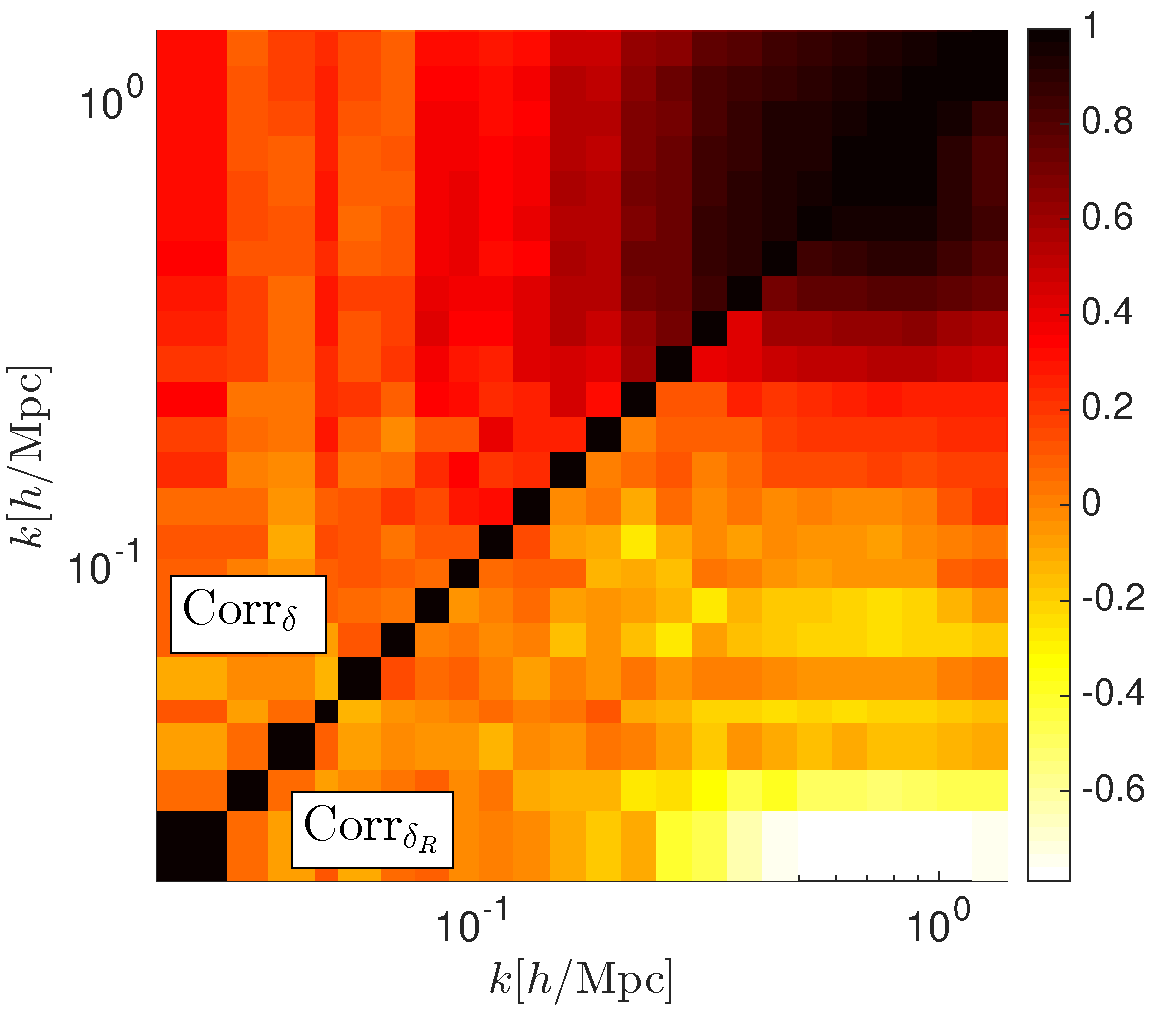
\includegraphics[width=0.48\textwidth]{corrmat_hot_2-crop.pdf}
%  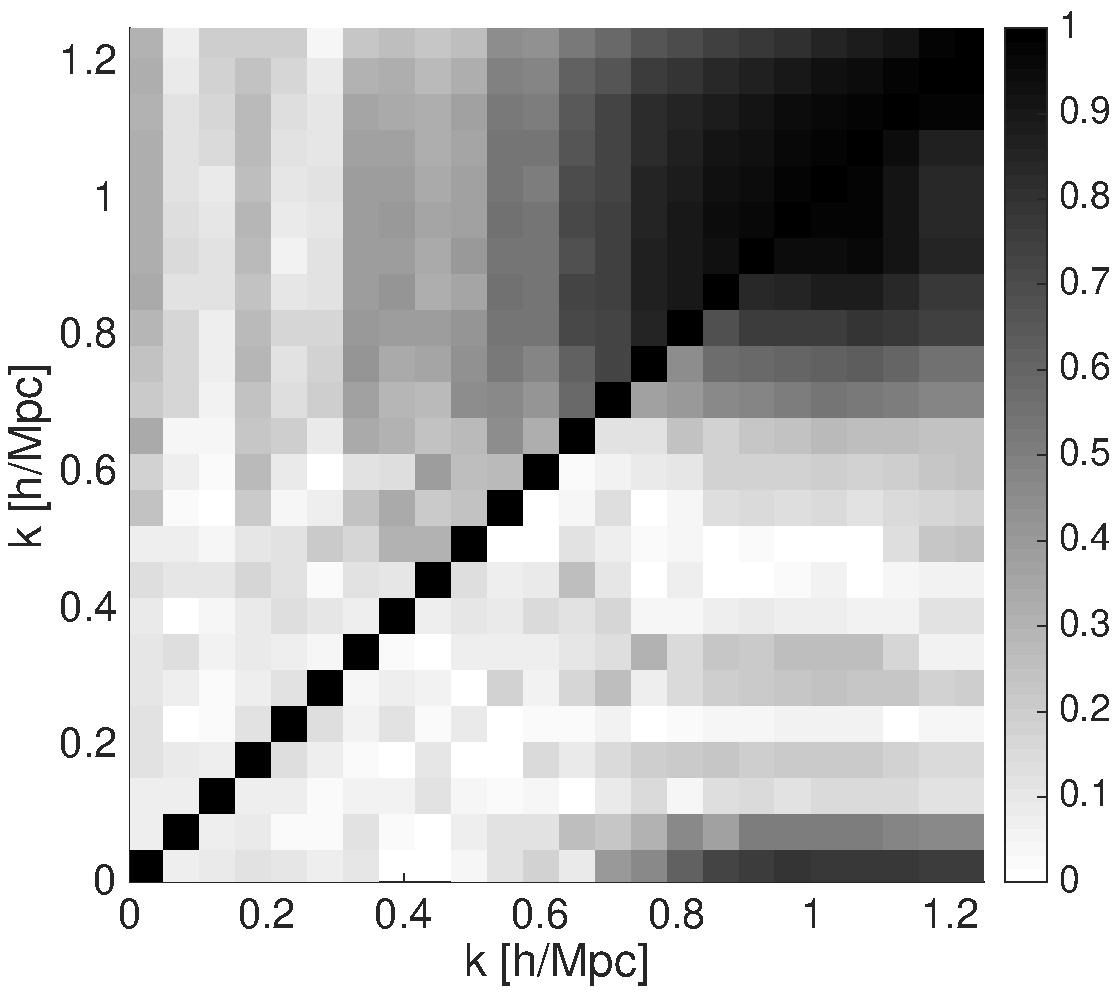
\includegraphics[width=0.48\textwidth]{corr_cut-crop.pdf}
  \caption{Correlation coefficient matrix as found from 136 non-linear power spectra 
(the upper-left elements) and the reconstructed power spectra (the lower-right off-diagonal elements). 
Both the matrix are symmetric and have unity diagonal elements.}
    \label{fig:corrall}
\end{figure}

%  The signal-to-noise ratio, sometimes also called Fisher information, can be given by the inverse matrix of covariance. Since the signal-to-noise ratio was given in some work, we also present it for a better comparison. 
%\begin{align}
%\left( \frac{S}{N}\right)^2 (k_{n}) =\sum_{i,j=1}^n P_i \mathrm{Cov}^{-1}(i,j) P_j
%\end{align}

  Cumulative Fisher information is proportional to the volume. We plot the 
cumulative Fisher information per $\mathrm{Mpc}^3/h$ of the non-linear, linear and reconstructed power specta in 
Fig.\ref{fig:fisherinfo}(a). The Fisher information of the non-linear power spectra drops 
from the linear one at $k \simeq$ 0.05 $h/\mathrm{Mpc}$, and has a flat plateau in the translinear regime, 
$k\simeq$ 0.3 $h/\mathrm{Mpc}$, with 
a saturated value of $I \simeq 2.5 \times 10^{-5}/(\mathrm{Mpc}^3/h^3)$. It 
indicates that there's nearly no independent information in the translinear regime of the power 
spectrum.
% At $k\sim0.8$, the information increase slightly aggain. 
But the information curve of 
the reconstructed power spectra keeps incresing roughly the same as 
the linear information until $k\simeq$ 0.3 $h/\mathrm{Mpc}$, and reaches it's plateau at $k\simeq$ 0.8 $h/\mathrm{Mpc}$ with the 
value of $I \simeq  10^{-3}/(\mathrm{Mpc}^3/h^3)$, up by a factor of  40. 
It indicates that the MM reconstructed method can strongly recover the lost information 
within this scale. We compare the Fisher information given by the MM reconstruction method with 
the logarithmic density mapping method \cite{bib:Mark2009} as an example to illustrate their strength. 
We find that the MM reconstruction gives more than 10 times more information than logarithmic mapping. 
In some papers, the cross-correlation $r^2$ terms are set to be unity in Eq. \ref{eq:fisherformulaused}, which 
apparantly increases the non-linear information. We also plot those in Fig. \ref{fig:fisherinfo}(b) 
for better comparison. But we find that in this case, the MM reconstructed and logarithmic mapping information in the scale 
$k \simeq$ 0.2 - 0.5 $h/\mathrm{Mpc}$ is higher than the linear one, which is not expected. 
\begin{figure*}
%\begin{subfigure}[b]{0.48\textwidth}
%\centering
  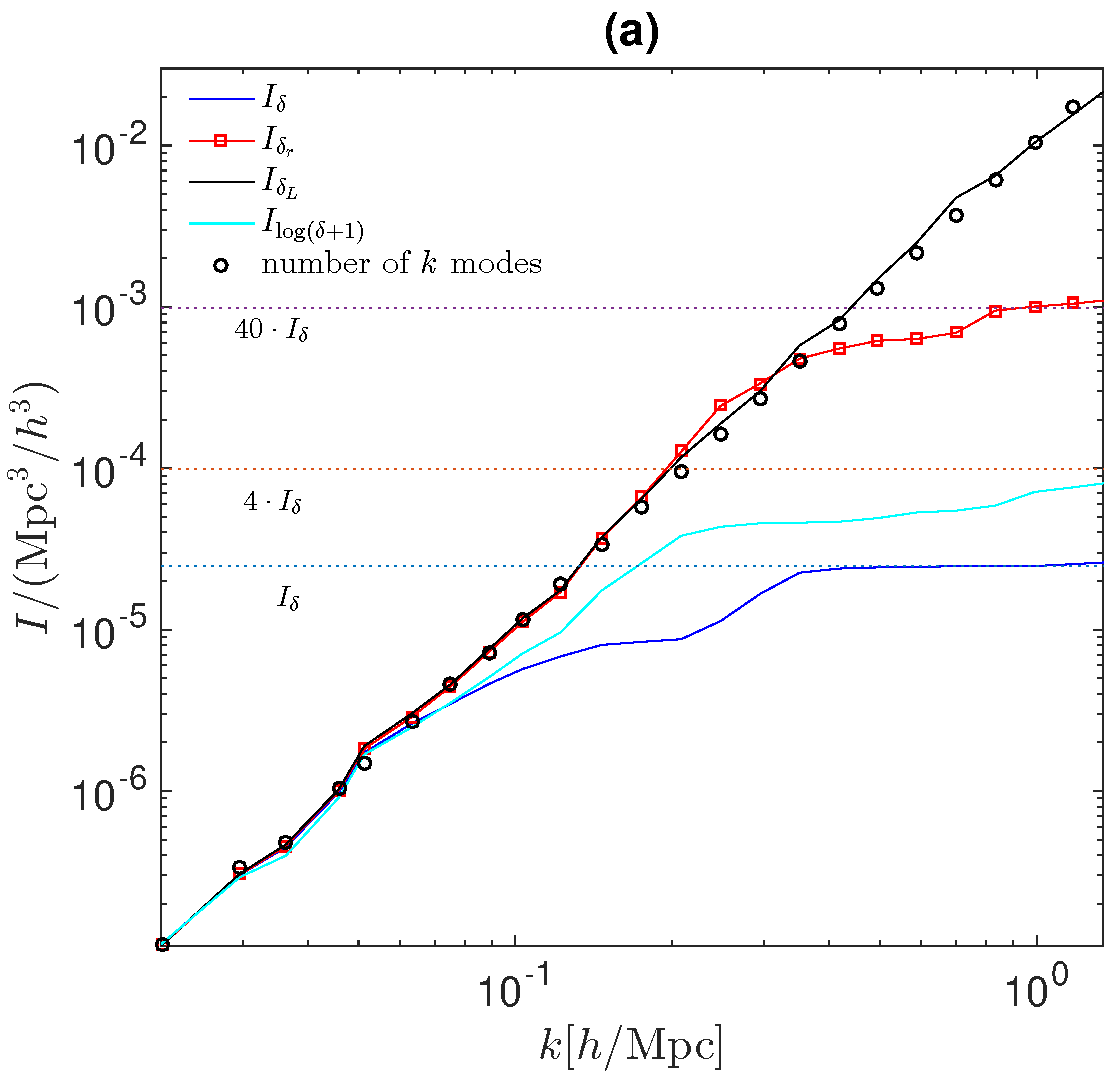
\includegraphics[width=0.5\textwidth]{fisher_r2_best_analysis-crop.pdf}
%\end{figure}
%\begin{subfigure}[b]{0.48\textwidth}
%\bebin{subfigure}
%\centering
  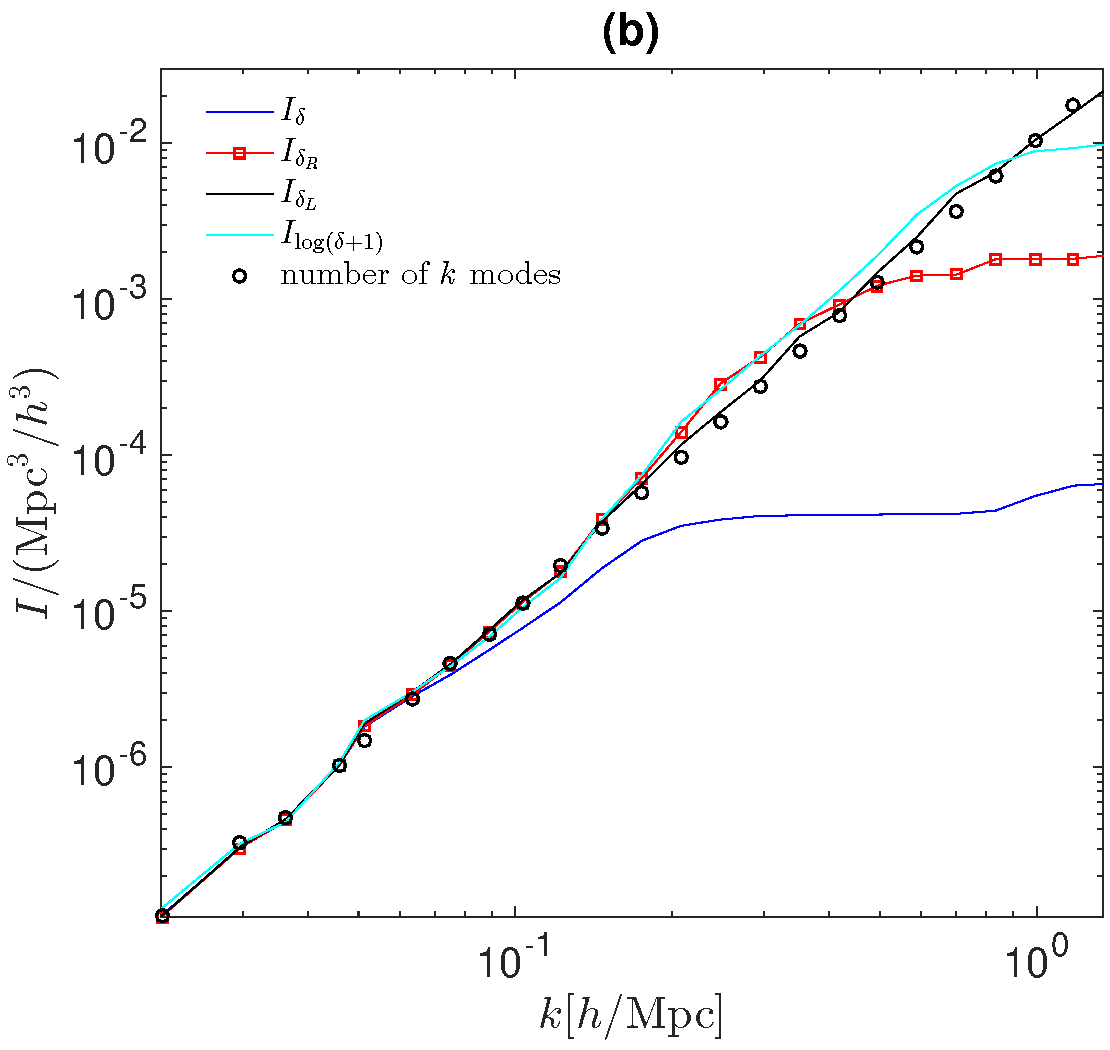
\includegraphics[width=0.46\textwidth]{fisher_best_analysis-crop.pdf}
%\end{subfigure}
%  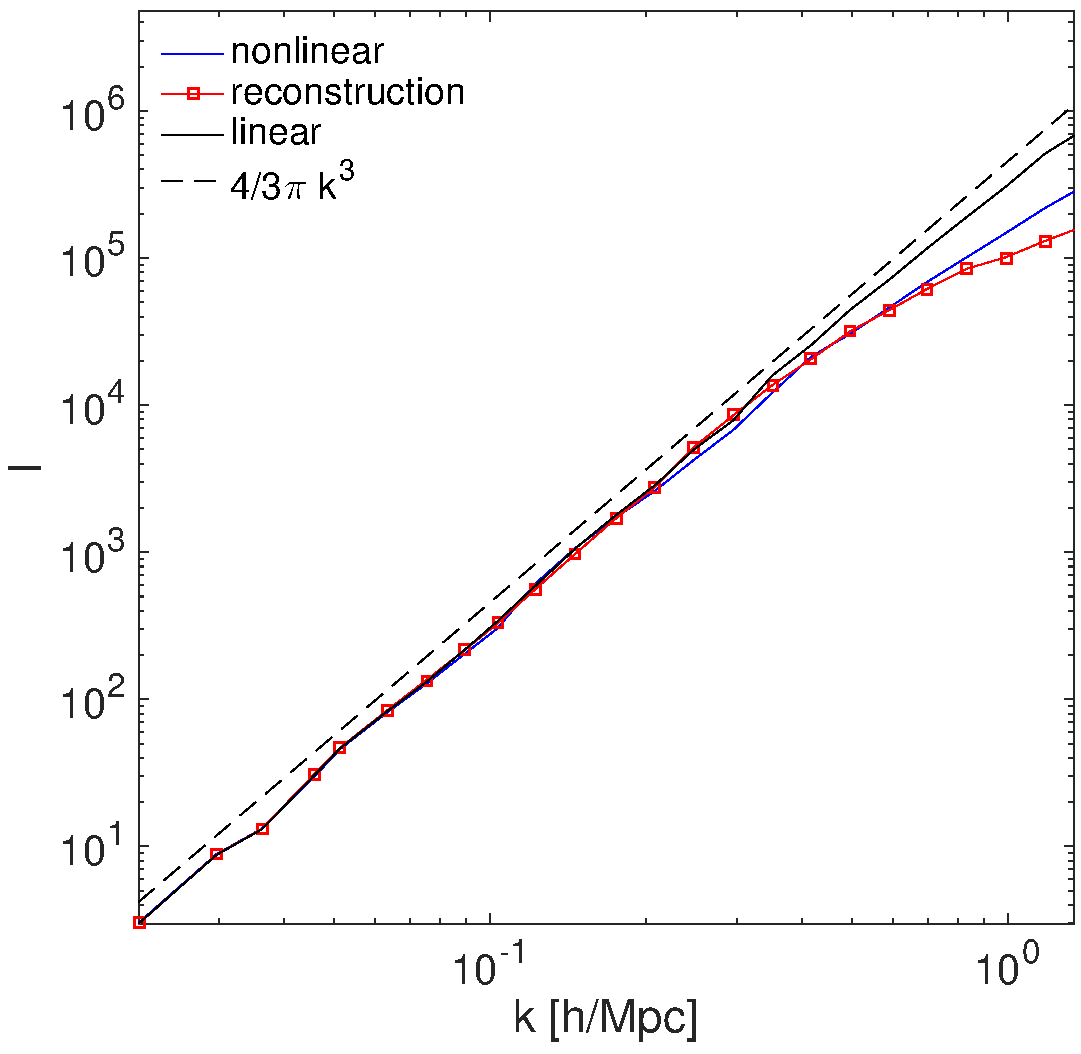
\includegraphics[width=0.48\textwidth]{fisher_tr-crop.pdf}
%  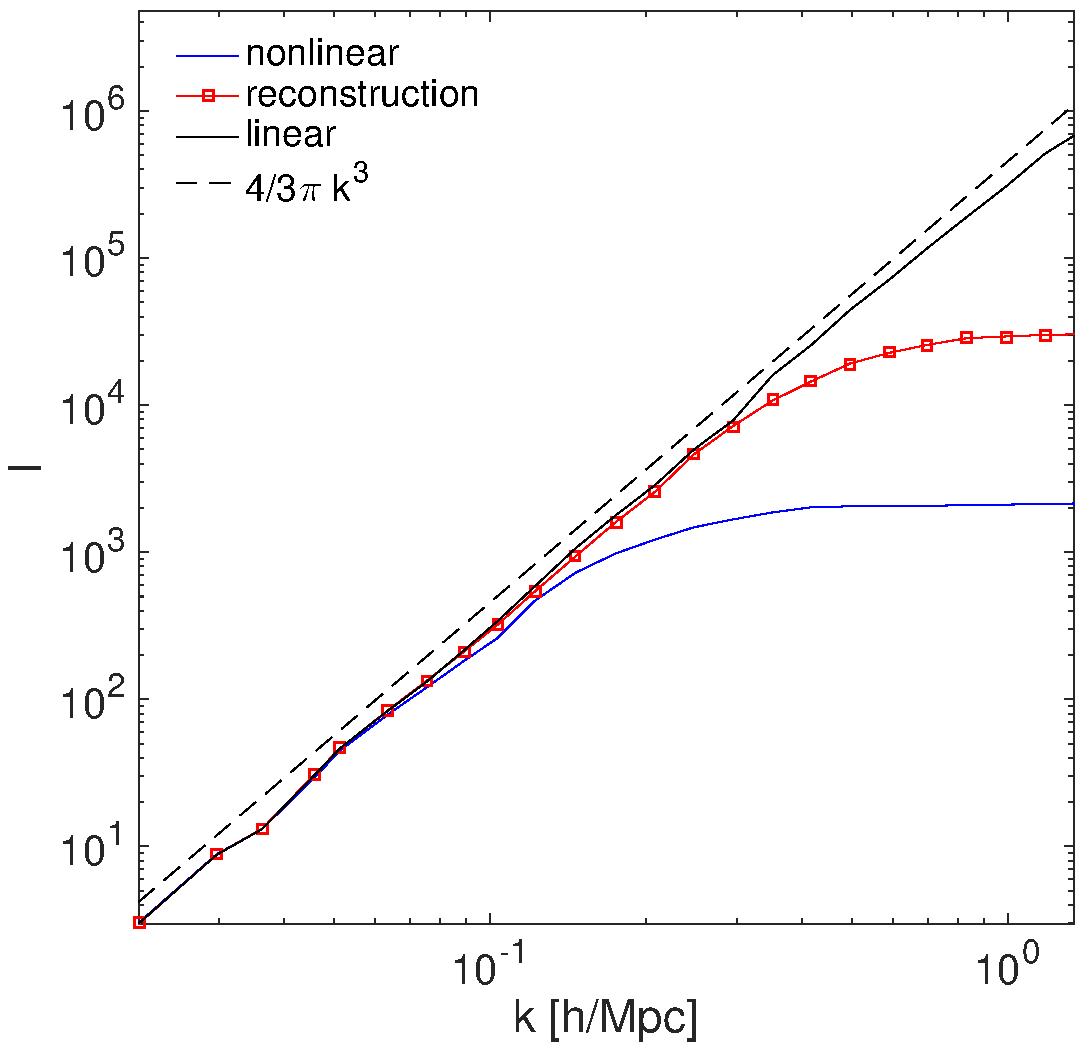
\includegraphics[width=0.48\textwidth]{fisher_trr2-crop.pdf}
\centering
   \caption{(a) Cumulative Fisher information per $\mathrm{Mpc}^3/h^3$ in the power spectra 
as a function of wavenumber. The blue line correspond to the non-linear density field; 
the red line with squares corresponds to the the reconstructed deformation 
potential; the dark line corresponds to the linear density field; the circles correspond to number 
of $k$ modes up to that wave bin. Dotted lines correspond to saturated value of 
non-linear Fisher information, 4 times and 40 times of it. (b) Cumulative Fisher information 
per $\mathrm{Mpc}^3/h^3$ given by setting the cross-correlation to be unity.}
  \label{fig:fisherinfo}

\end{figure*}
%\begin{figure*}
%[htbp]
% \centering
%  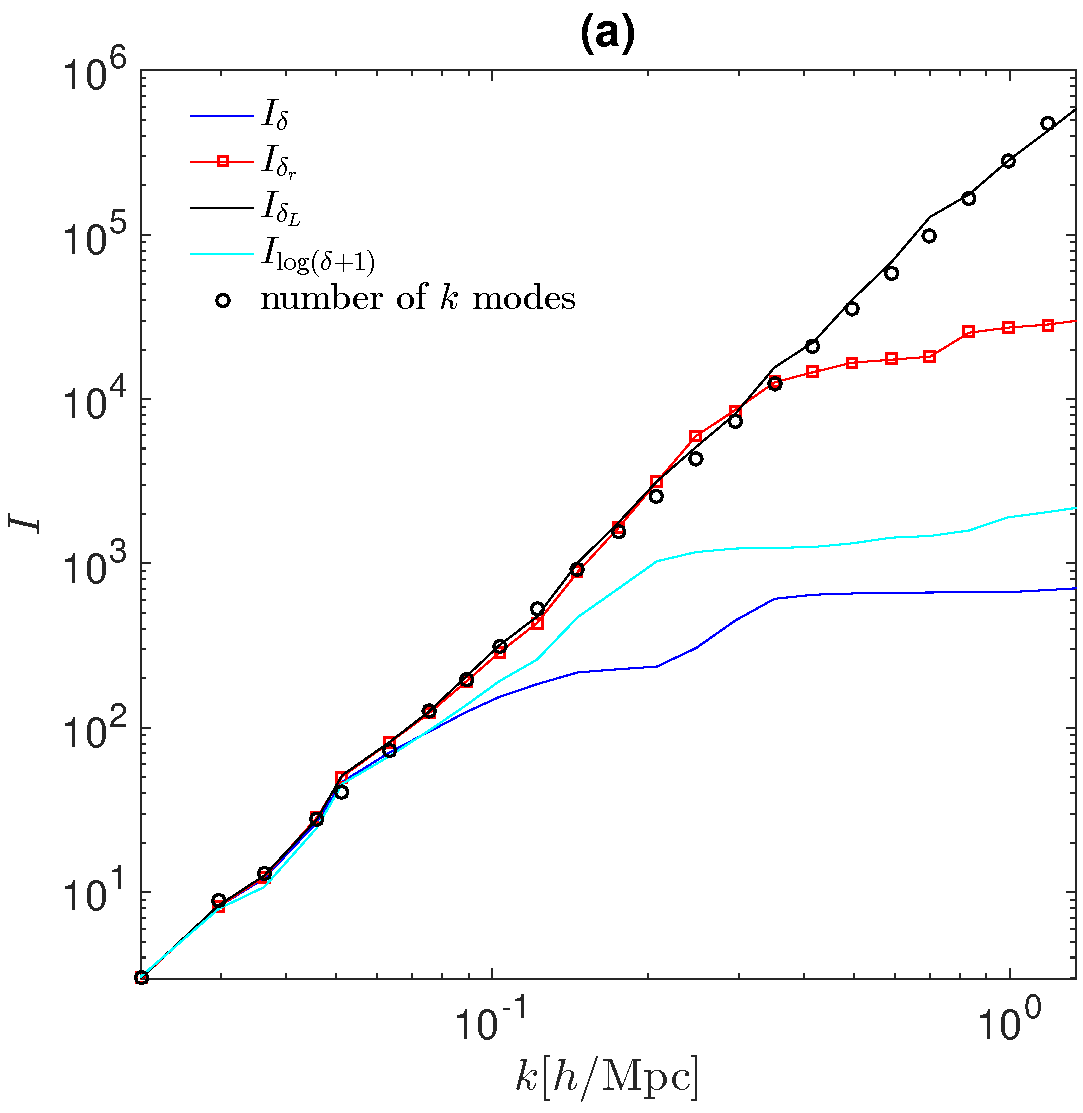
\includegraphics[width=0.48\textwidth]{fisher_addlog_r2-crop.pdf}
%  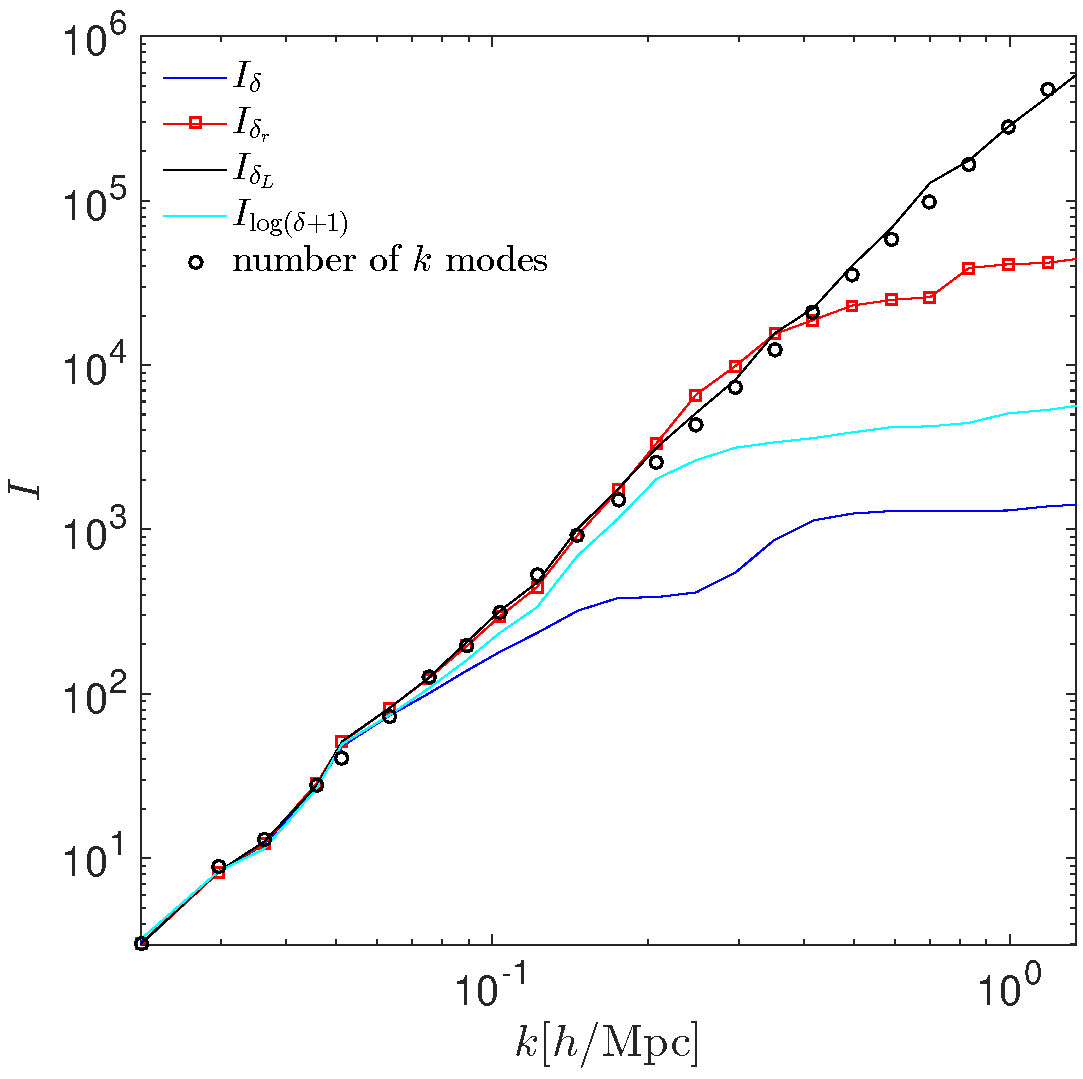
\includegraphics[width=0.48\textwidth]{fisher_addlog_r-crop.pdf}
%  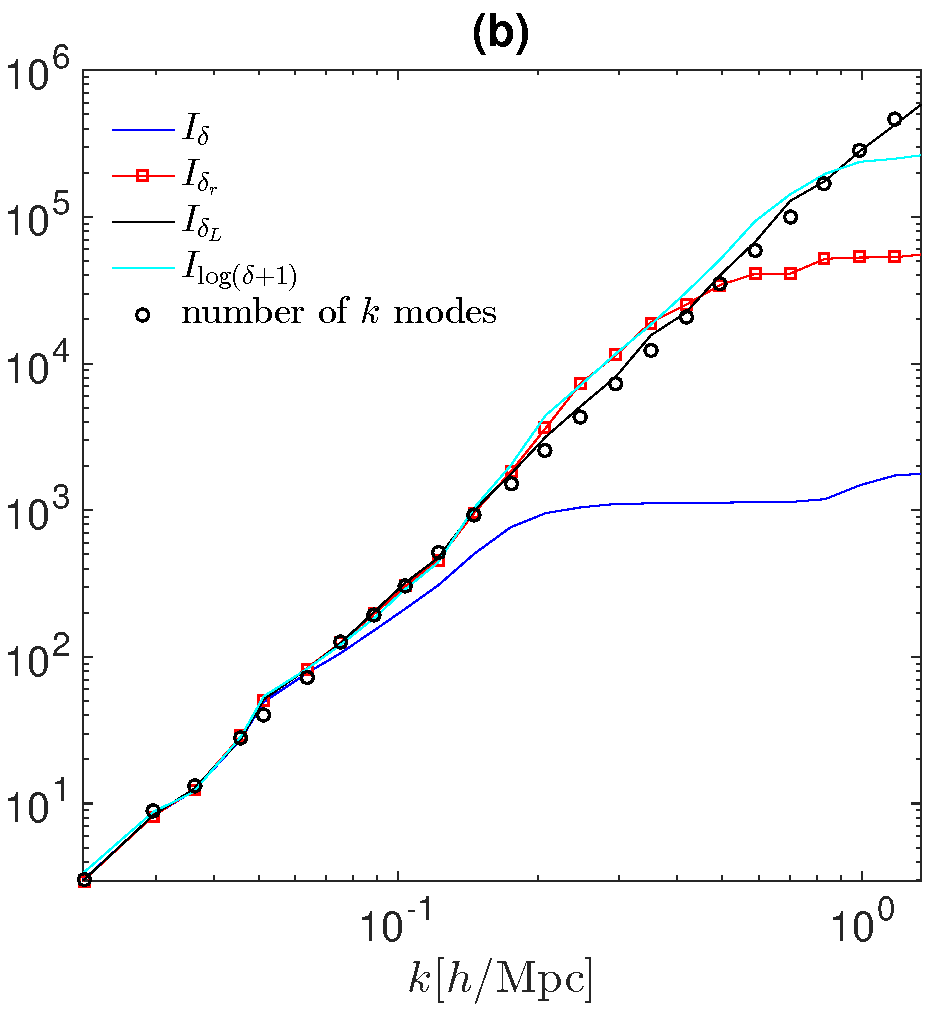
\includegraphics[width=0.48\textwidth]{fisher_addlog-crop.pdf}
%\caption{1:$r^2$; 2:$r$; 3:old version}
%  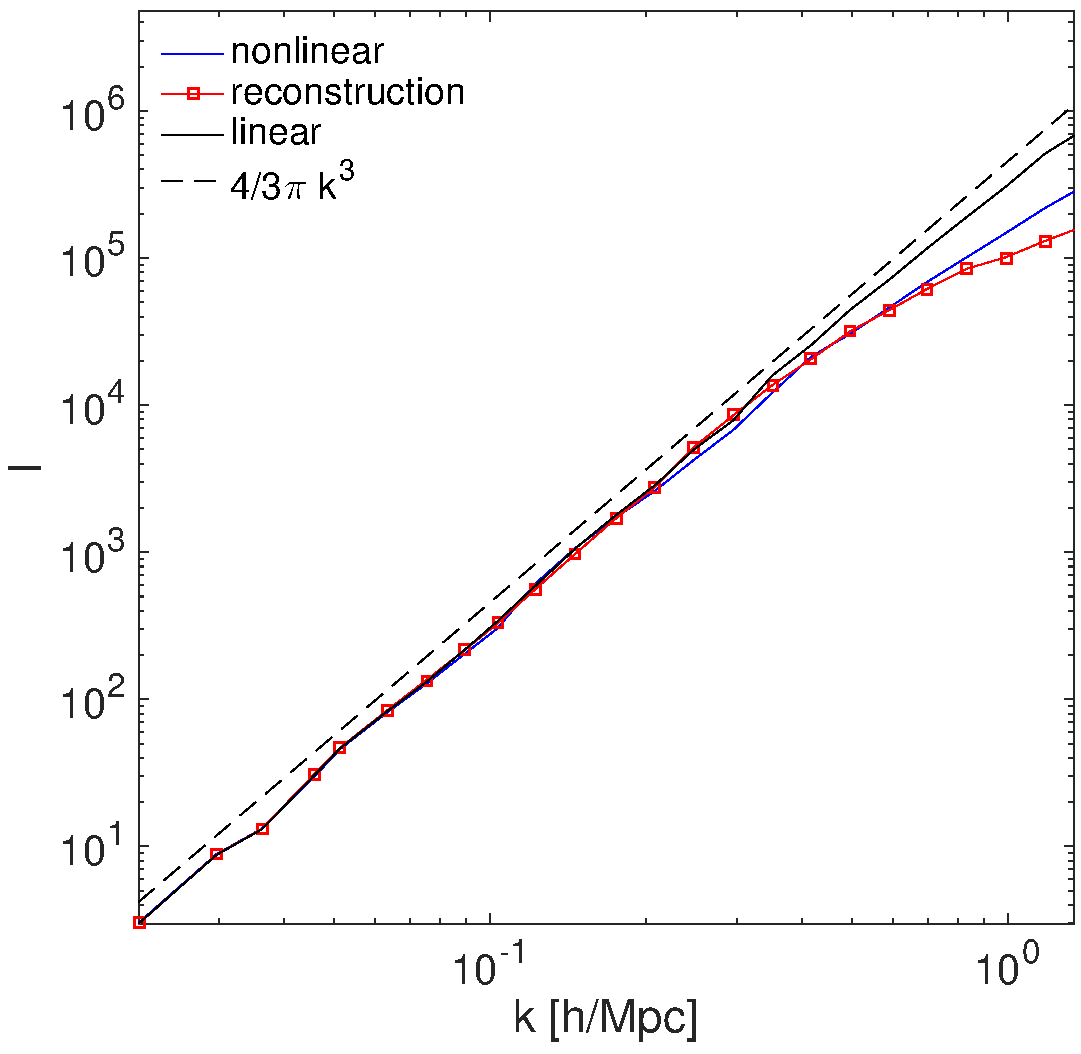
\includegraphics[width=0.48\textwidth]{fisher_tr-crop.pdf}
%  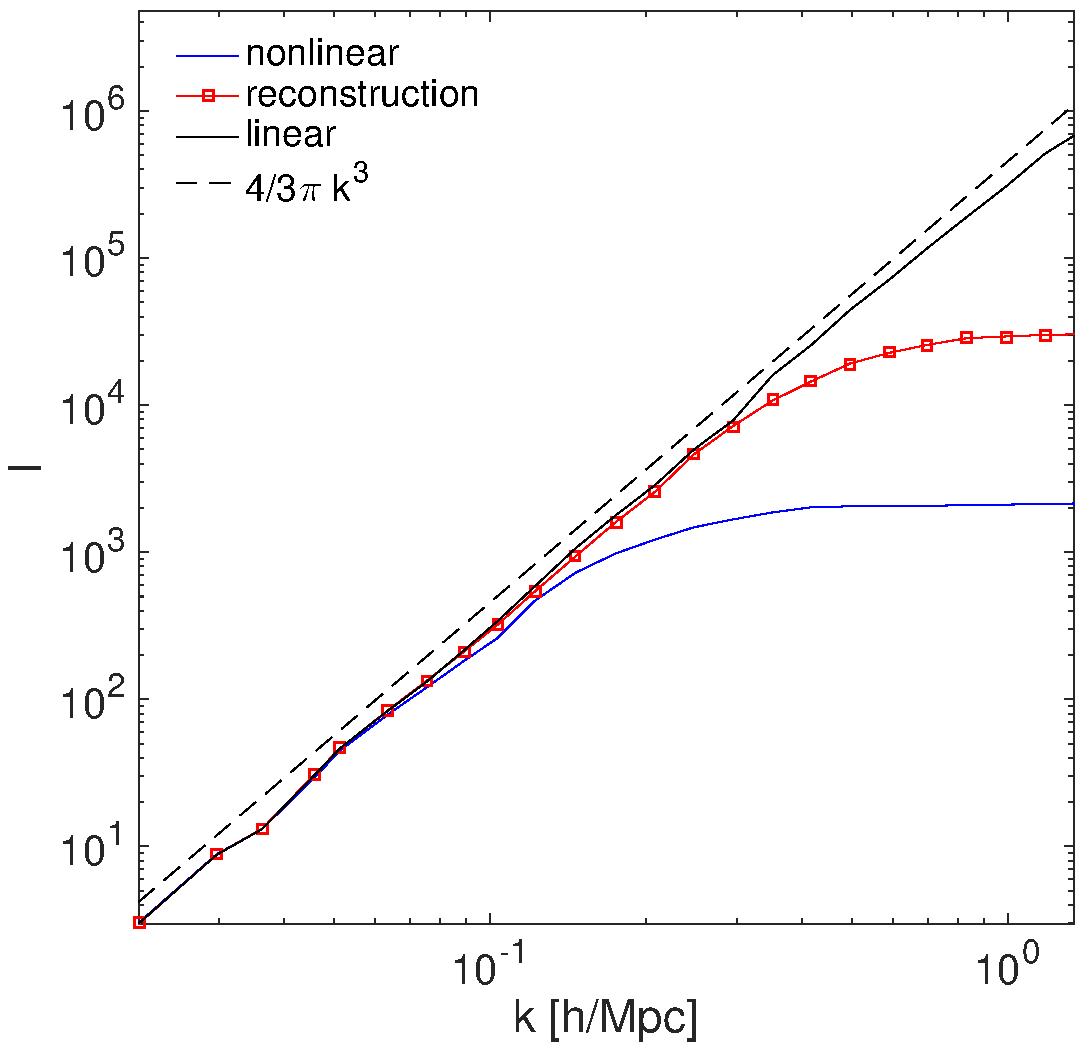
\includegraphics[width=0.48\textwidth]{fisher_trr2-crop.pdf}
%\end{figure*}
%\begin{figure*}
%\centering
%  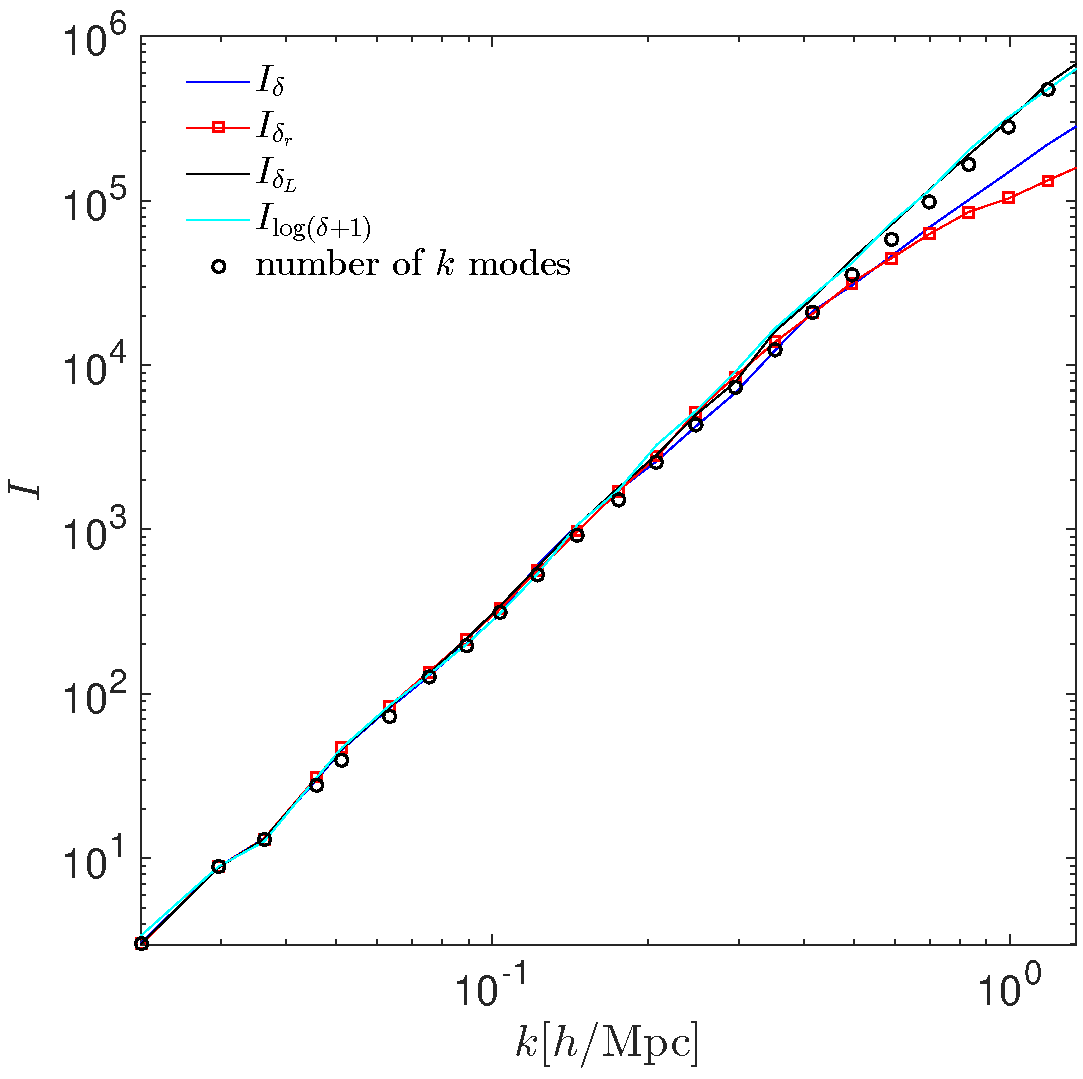
\includegraphics[width=0.48\textwidth]{fisher_addlog_diag-crop.pdf}
%  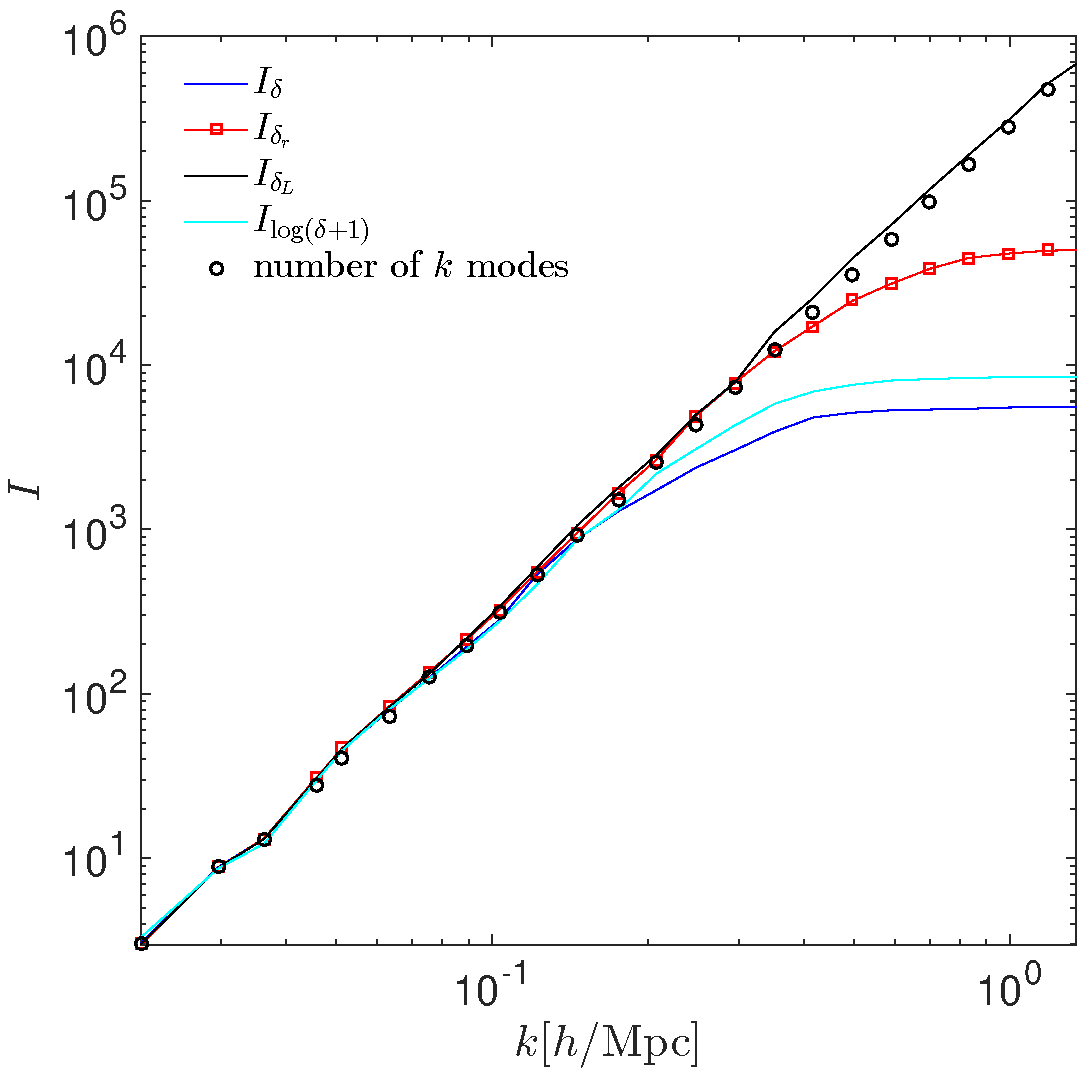
\includegraphics[width=0.48\textwidth]{fisher_addlog_diagr-crop.pdf}
%  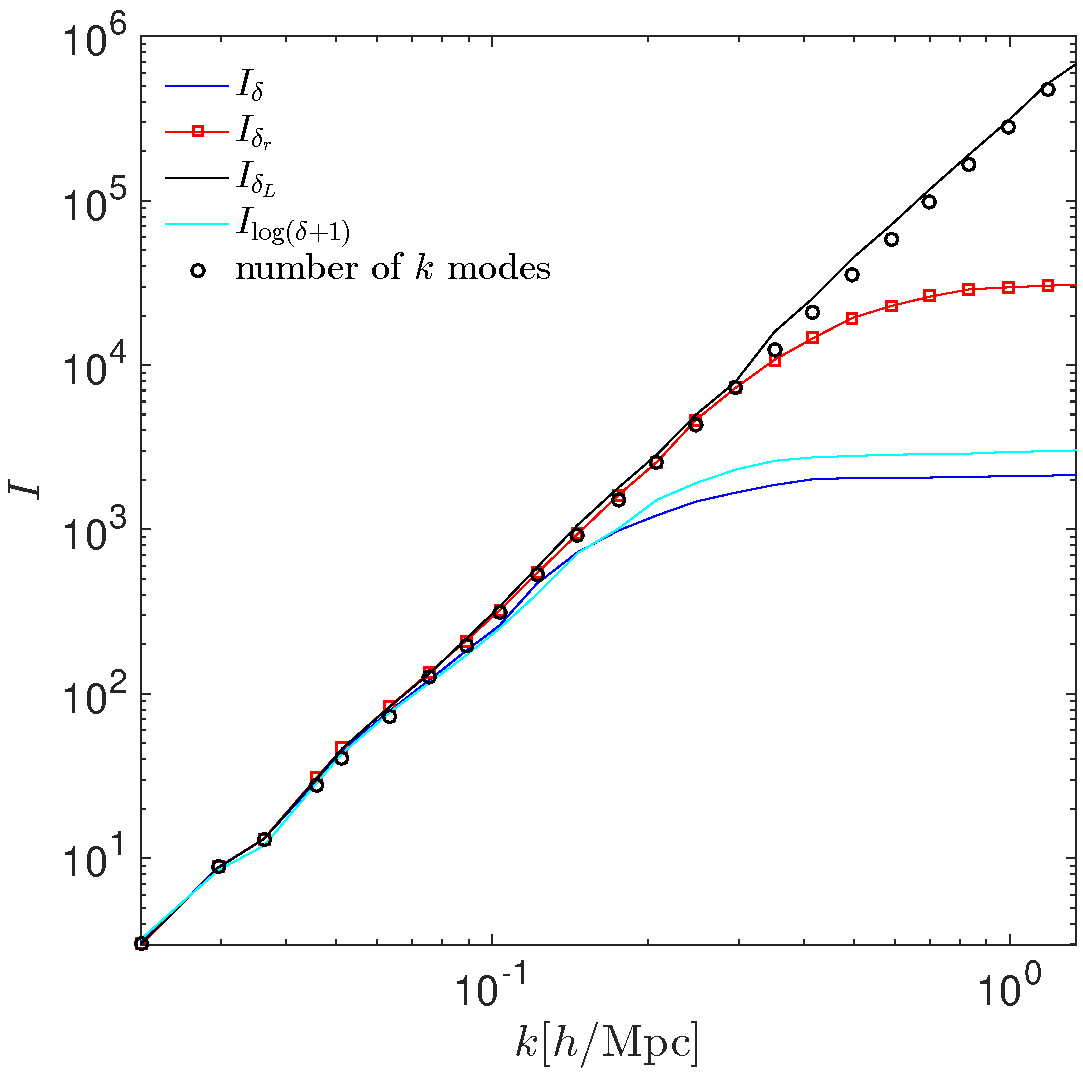
\includegraphics[width=0.48\textwidth]{fisher_addlog_diagr2-crop.pdf}
%\caption{1: diag; 2: diag*$r$, 3: diag*$r^2$}
%\end{figure*}

\end{section}


\begin{section}{Conclusion}
  \label{sec:conclusion}
  The MM reconstruction method successfully recovers the lost linear
  information on mildly non-linear scales and increases the saturated
  information from $I \simeq 2.5 \times 10^{-5}/(\mathrm{(Mpc/h)}^3)$
  to at least $I \simeq 10^{-3}/(\mathrm{(Mpc/h)}^3)$.  The result is
  better than previous methods,
  e.g. \cite{bib:Mark2006,bib:Mark2009,bib:Zhang2011,bib:Yu2012}, and
  we may improve further as the correlation coefficient between the
  reconstructed and linear fields will increase with higher resolution
  simulations \cite{bib:ZhuH2016}.  This successful result on cold
  dark matter density fields provides strong motivation to adapt the
  MM reconstruction scheme to other cosmological fields such as biased
  tracers like halos and other matter components like baryons and
  neutrinos.

  % The result in dark matter density fields gives a strong motivation
  % to adapt the MM reconstruction to halo fields, neutrino fields,
  % etc, so that we have access to the physics in smaller scales.

  % Reconstruction technique are concerned to improve cosmology
  % measurements of BAO scale
  % (e.g. \cite{bib:Daniel2007,bib:Martin2015}).  The successful
  % application of the MM reconstruction on BAO reconstruction in 1D
  % \cite{bib:Zhu2016} and 3D \cite{bib:ZhuH2016} cosmology provide an
  % intuitive view of the algorithm to push forward BAO research.

  % The MM reconstruction effectively decomposes the irrotational part
  % and the curl part of the displacement field of particles. However,
  % the reconstructed displacement might be greatly different from the
  % real displacement in N-body simulation, since it is sensitive to
  % the
  % late stage shell-crossing and nonlinear process so that the
  % original
  % position of some spectific particles are replaced by each other.
  % It
  % is meaningful to compare the irrotational displacement field
  % through
  % the MM reocnstruction and through $E$-mode displacement
  % reconstruction \cite{bib:Yu2016}.  Since the MM reconstruction
  % only
  % needs the density field input and gives a large amount of
  % recovering
  % of lost information, it's expected to have a good effect on
  % reconstructing the matter density field from observation.
\end{section}


\acknowledgements{
  \label{sec:acknowledgements}
  We thank Homg-Ming Zhu and Xin Wnag for friendly and helpful discussion.  Computations were performed on
  the General Purpose Cluster supercomputer at the SciNet HPC
  Consortium.  SciNet is funded by: the Canadian Foundation for
  Innovation under the auspices of Compute Canada; the Government of
  Ontario; Ontario Research Fund - Research Excellence; and the
  University of Toronto.  
}


\bibliographystyle{apsrev}
\bibliography{myreference}
\widetext
\clearpage
%\input{./supplement.tex}

\end{document}
